\documentclass[a4paper,oneside,onecolumn]{article}
\usepackage[utf8x]{inputenc}
\usepackage[T1]{fontenc}
\usepackage{mathtools}
\usepackage{color}
\usepackage{siunitx}
\usepackage{microtype}
\usepackage{fancyhdr}
\usepackage{amsmath}
\usepackage{listings}
\usepackage[T1]{fontenc}
\usepackage{amssymb}
\usepackage{}
\usepackage[head=12pt,hmargin=2.5cm,vmargin=2.5cm]{geometry}

\renewcommand*\lstlistingname{Code Snippet}

\definecolor{codegreen}{rgb}{0,0.6,0}
\definecolor{codegray}{rgb}{0.5,0.5,0.5}
\definecolor{codepurple}{rgb}{0.58,0,0.82}
\definecolor{backcolour}{rgb}{0.95,0.95,0.92}

\lstdefinestyle{mystyle}{
    backgroundcolor=\color{backcolour},   
    commentstyle=\color{codegreen},
    keywordstyle=\color{magenta},
    numberstyle=\tiny\color{codegray},
    stringstyle=\color{codepurple},
    basicstyle=\footnotesize,
    breakatwhitespace=false,         
    breaklines=true,                 
    captionpos=b,                    
    keepspaces=true,                 
    numbers=left,                    
    numbersep=5pt,                  
    showspaces=false,                
    showstringspaces=false,
    showtabs=false,                  
    tabsize=2
}
 
\lstset{style=mystyle}

\DisableLigatures[>,<]{encoding = T1,family=tt*} %

\definecolor{codegray}{gray}{0.9}
\newcommand{\code}[1]{\colorbox{codegray}{\texttt{#1}}}

\pagestyle{fancy}

\begin{document}

\title{Lab 4 \\ Kernel Patching and Cross-Compilation for RPi \\ Embedded Linux}
\author{Julia Desmazes \\ Michael Nissen}
\date{\today}
\maketitle
\bigskip

\section{Download / Set the good version of Linux sources}

\noindent
To execute the tasks for this report, the first step is to get the Raspberry Pi cross-compilation tools, and specific version of the linux kernal that one wants to patch. This is going to be done using \code{git clone}, which ofcourse assumes a working installation of \texttt{git}.
\newline
To get the latest version of the kernel source code and the cross-compilation tools, the following commands with be copied to the terminal:
\begin{lstlisting}
host$ git clone https://github.com/raspberrypi/tools.git
host$ git cone -b rpi-4.4.y https://github.com/raspberrypi/linux.git
\end{lstlisting}
One now has to make sure to get the same configuration as is used by ones Raspberry Pi during the kernel compilation, which can be done by checking out the \texttt{git branch} that corresponds to the hash of the Linux kernel running on the Raspberry Pi.
\newline
This will be done by by running the shells script seen in Code Snippet \ref{lst:git_hash}. This shell script will grep the firmware hash found on the Raspberry pi, and then get the \texttt{git hash} from the github link relative to the hardware hash.
\begin{lstlisting}[caption={Shell script to get Linux kernel git hash}, label={lst:git_hash}]
#!/bin/bash

PLATFORM=`uname -s` 

if [ ${PLATFORM} = "Darwin" ]
then
    CMD="gunzip -c"
elif [ ${PLATFORM} = "Linux" ]
then
    CMD="zcat"
else
    echo "Sorry, the platform ${PLATFORM} is not supported !!!"    
    exit -1
fi

FWHASH=`${CMD} /usr/share/doc/raspberrypi-bootloader/changelog.Debian.gz | grep -m 1 'as of' | awk '{print $NF}'`
#echo "Firmware Hashcode: fwhash = $FWHASH"

LINUXHASH=`wget -qO- https://raw.github.com/raspberrypi/firmware/$FWHASH/extra/git_hash`

echo "Linux Hashcode: linuxhash = $LINUXHASH"
\end{lstlisting}
When one has figured out the \texttt{git hash}, one can change directory to the linux git repository and checkout the respective brach by the following command:
\begin{lstlisting}
host$ cd linux
host$ git checkout <git_hash>
host$ make clean -mrproper
\end{lstlisting}
At line 3, we are cleaning kernel tree from all unneeded files of the first version which is a recommended practice prior to each kernel compilation!

\section{Patch the Kernel}

\noindent
Before starting to patch the kernel, one should make sure to identify the Linux sources that one is trying to install. This can be done using the \code{head} command, which will look like this:
\begin{lstlisting}
host$ head Makefile

	# Ouput generated by running head on the Makefile #
	VERSION = 4
	PATCHLEVEL = 4
	SUBLEVEL = 21
	EXTRAVERSION = 
	NAME = Blurry Fish Butt
\end{lstlisting}
Now that one know the specific version of the Linux kernel, it is time to download the latest \texttt{PREMEPT-RT} patch that corresponds to ones kernel version - if follows the format: \texttt{version.patch-level.sub-level}.
\newline
To download the patch from the patch from \texttt{kernel.org} using the \code{wget} command like so: 
\newline
\code{wget https://cd.kernel.org/pub/linux/kernel/projects/rt/4.9/patch-4.9.47-rt47.patch.gz}
\newline
\newline
Now one can actually start patching the kernel sources by executing the following commands in succession:
\begin{lstlisting}
host$ gunzip patch-<version.patch-level.sub-level>-rt<last>.patch.gz
host$ cat patch-<version.patch-level.sub-level>-rt<last>.patch | patch -p1
\end{lstlisting}
One can now create a folder named \texttt{rt-modules} under your project folder - at the same level as the \texttt{linux} and \texttt{tools} folders, and export an environment variable \texttt{INSTALL\_MOD\_PATH} that points to that folder:
\begin{lstlisting}
host$ mkdir rt-modules
host$ cd rt-modules
host$ export INTALL_MOD_PATH=$PWD
\end{lstlisting}
Here \code{\$PWD} is the path to the current directory.

\section{Configure Cross-compilation}

Before starting the cross-compilation, one is going to specify the architecture for which to compile, the cross-compiler that ones wishes to use, and the kernel that one is trying to compile for. This is done by exporting some specific environment variables that is used by the makefile:
\begin{lstlisting}
host$ export ARCH=arm KERNEL=kernel7
host$ export CROSS_COMPILE=$PWD/tools/arm-bcm2708/gcc-linaro-arm-linux-gnueabihf-raspbian-x64/arm-linux-gnueaihf-
\end{lstlisting}
Now, to configure the kernel in an appropriate way, one can use the existing kernel configuration from the Raspberry Pi. This configuration file can be generatied using the \code{modprobe} command, and then copy that generated file from the Raspberry Py over to the \texttt{linux/} folder on the host machine using the \code{scp} command. Finaly, extract the content of the \texttt{config.gz} into a \texttt{.config} file:
\begin{lstlisting}
host$ sudo modprobe configs
host$ scp pi@193.169.0.26:/proc/config.gz /home/user/kernel_labs/linux
host$ zcat -c config.gz > .config
\end{lstlisting}
Now that one has created a default \texttt{.config} file, it is time to costumise the kernel using the \code{sudo make menuconfig} which opens the GUI seen in Figure \ref{fig:menuconfig}. For the purpose of this lab assignment, we are going to enable the \texttt{Fully Preemptible Kernel} setting, and the \texttt{High Resolution Timer Support}.
\begin{figure}[htbp]
	\centering
	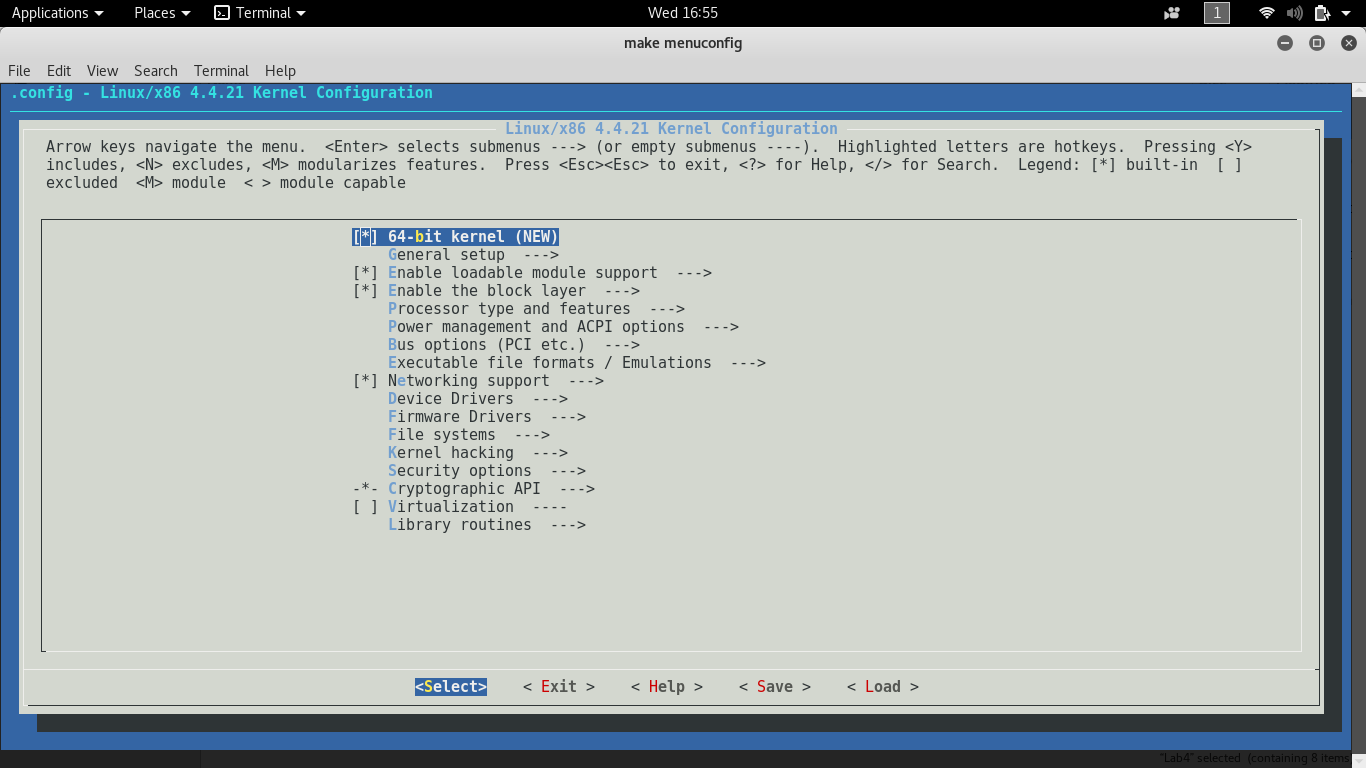
\includegraphics[width=0.95\textwidth]{resources/meunconfig.png}
	\caption{The \texttt{menuconfig} GUI}
	\label{fig:menuconfig}
\end{figure}

\newpage
\section{Build the new Kernel and Modules}

To build the kernel,

\end{document}